\documentclass[10pt]{article}

\usepackage[paperwidth=210mm,paperheight=225mm,
  textwidth=180mm,textheight=215mm,top=5mm]{geometry}
\usepackage{amsmath,array,tabularx,tikz,xcolor}
\usetikzlibrary{arrows.meta,calc,positioning}
\pagestyle{empty}

\definecolor{accent}{HTML}{A51C30}
\definecolor{charcoal}{HTML}{242424}
\definecolor{softgray}{HTML}{F3F3F3}

\begin{document}
\centering
\hyphenpenalty=10000
\exhyphenpenalty=10000

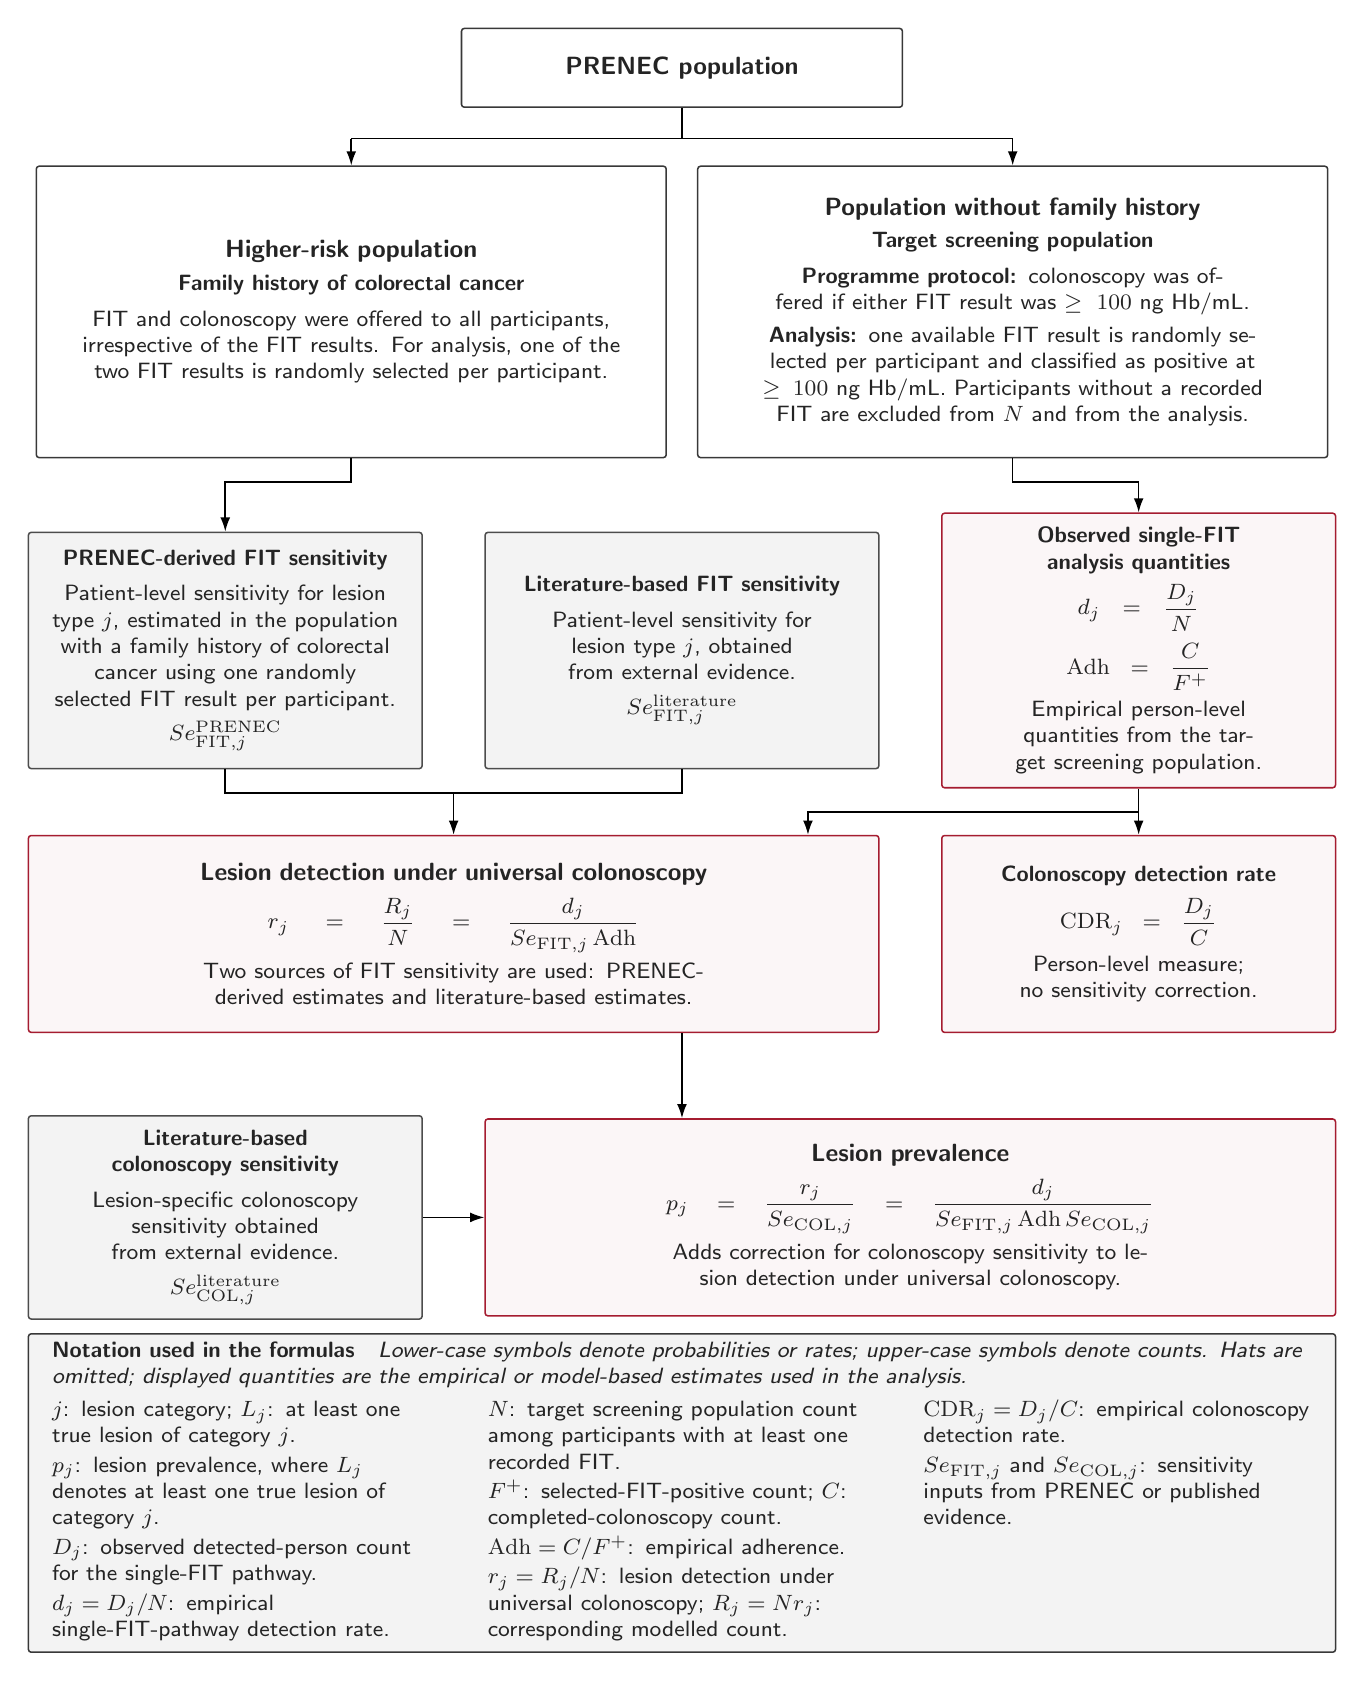
\begin{tikzpicture}[
  x=1mm,
  y=1mm,
  >={Latex[length=1.8mm,width=1.25mm]},
  every node/.style={font=\sffamily, text=charcoal},
  flow/.style={-{Latex[length=1.8mm,width=1.25mm]}, line width=0.58pt},
  bus/.style={line width=0.58pt},
  box/.style={draw=black!78, fill=white, line width=0.55pt,
    rounded corners=1pt, align=center, inner xsep=3mm, inner ysep=1.8mm},
  programme/.style={box, text width=50mm, minimum height=10mm,
    font=\sffamily\small\bfseries},
  population/.style={box, text width=74mm, minimum width=80mm,
    minimum height=37mm,
    font=\sffamily\footnotesize},
  source/.style={box, draw=accent, fill=accent!4,
    text width=44mm, minimum width=50mm,
    minimum height=30mm,
    font=\sffamily\footnotesize},
  sensitivity/.style={box, draw=black!70, fill=softgray,
    text width=44mm, minimum width=50mm,
    minimum height=30mm,
    font=\sffamily\footnotesize},
  sensitivityside/.style={box, draw=black!70, fill=softgray,
    text width=44mm, minimum width=50mm,
    minimum height=25mm,
    font=\sffamily\footnotesize},
  external/.style={source},
  adjustedbox/.style={box, draw=accent, fill=accent!4,
    text width=102mm, minimum width=108mm,
    minimum height=25mm,
    font=\sffamily\footnotesize},
  sidebox/.style={box, draw=accent, fill=accent!4,
    text width=44mm, minimum width=50mm,
    minimum height=25mm,
    font=\sffamily\footnotesize},
  notation/.style={box, fill=softgray, text width=160mm,
    minimum width=166mm, minimum height=34mm,
    align=left, inner ysep=1.0mm, font=\sffamily\footnotesize}
]

% Fixed three-column grid:
%   x = -58 mm, 0 mm, +58 mm for source boxes;
%   all boxes in a row share the same vertical centre.

% PRENEC population and family-history split.
\node[programme] (prenec) at (0,0) {PRENEC population};

\node[population] (familyhistory) at (-42,-31) {%
  {\small\bfseries Higher-risk population}\\[0.8mm]
  {\bfseries Family history of colorectal cancer}\\[1.2mm]
  FIT and colonoscopy were offered to all participants, irrespective of the FIT
  results. For analysis, one of the two FIT results is randomly selected per
  participant.
};

\node[population] (nofamilyhistory) at (42,-31) {%
  {\small\bfseries Population without family history}\\[0.8mm]
  {\bfseries Target screening population}\\[1.2mm]
  {\bfseries Programme protocol:} colonoscopy was offered if either FIT result was
  $\geq100$ ng Hb/mL.\\[0.8mm]
  {\bfseries Analysis:} one available FIT result is randomly selected per
  participant and classified as positive at $\geq100$ ng Hb/mL. Participants
  without a recorded FIT are excluded from $N$ and from the analysis.
};

\coordinate (popsplit) at (0,-9);
\draw[bus] (prenec.south) -- (popsplit);
\draw[bus] (popsplit -| familyhistory.north) --
  (popsplit -| nofamilyhistory.north);
\draw[flow] (popsplit -| familyhistory.north) -- (familyhistory.north);
\draw[flow] (popsplit -| nofamilyhistory.north) -- (nofamilyhistory.north);

% Aligned source row.
\node[sensitivity] (localfit) at (-58,-74) {%
  {\bfseries PRENEC-derived FIT sensitivity}\\[1.2mm]
  Patient-level sensitivity for lesion type $j$, estimated in the population
  with a family history of colorectal cancer using one randomly selected FIT
  result per participant.\\[1.0mm]
  $Se^{\mathrm{PRENEC}}_{\mathrm{FIT},j}$
};

\node[sensitivity] (literaturefit) at (0,-74) {%
  {\bfseries Literature-based FIT sensitivity}\\[1.2mm]
  Patient-level sensitivity for lesion type $j$, obtained from external
  evidence.\\[1.0mm]
  $Se^{\mathrm{literature}}_{\mathrm{FIT},j}$
};

\node[source] (observed) at (58,-74) {%
  {\bfseries Observed single-FIT analysis quantities}\\[1.0mm]
  $\displaystyle d_j=\frac{D_j}{N}$\\[1.2mm]
  $\displaystyle \mathrm{Adh}=\frac{C}{F^+}$\\[1.0mm]
  Empirical person-level quantities from the target screening population.
};

\draw[flow] (familyhistory.south) -- ++(0,-3mm) -| (localfit.north);
\draw[flow] (nofamilyhistory.south) -- ++(0,-3mm) -| (observed.north);

% Aligned estimand row: modelled route on the left, descriptive route on the right.
\node[adjustedbox] (adjusted) at (-29,-110) {%
  {\small\bfseries Lesion detection under universal colonoscopy}\\[1.2mm]
  $\displaystyle r_j=\frac{R_j}{N}
    =\frac{d_j}{Se_{\mathrm{FIT},j}\,\mathrm{Adh}}$\\[1.0mm]
  Two sources of FIT sensitivity are used: PRENEC-derived estimates and
  literature-based estimates.
};

\node[sidebox] (colonoscopycdr) at (58,-110) {%
  {\bfseries Colonoscopy detection rate}\\[1.2mm]
  $\displaystyle \mathrm{CDR}_j
    =\frac{D_j}{C}$\\[1.0mm]
  Person-level measure; no sensitivity correction.
};

% The two FIT-sensitivity sources merge symmetrically before entering the
% adjusted estimate. Observed data then branch to the modelled and descriptive
% routes through a single junction.
\coordinate (fitlane) at ($(localfit.south)+(0,-3mm)$);
\coordinate (fitjoin) at (fitlane -| adjusted.north);
\coordinate (adjfit) at (adjusted.north);
\coordinate (rightportx) at (16,0);
\coordinate (adjobs) at (adjusted.north -| rightportx);
\coordinate (obsbranch) at ($(observed.south)+(0,-3mm)$);

\draw[bus] (localfit.south) -- (fitlane) -- (fitjoin);
\draw[bus] (literaturefit.south) -- ++(0,-3mm) -- (fitjoin);
\draw[flow] (fitjoin) -- (adjfit);
\draw[bus] (observed.south) -- (obsbranch);
\draw[flow] (obsbranch) -| (adjobs);
\draw[flow] (obsbranch) -- (colonoscopycdr.north);

% Aligned prevalence row.
\node[sensitivityside] (literaturecol) at (-58,-146) {%
  {\bfseries Literature-based colonoscopy sensitivity}\\[1.2mm]
  Lesion-specific colonoscopy sensitivity obtained from external
  evidence.\\[1.0mm]
  $Se^{\mathrm{literature}}_{\mathrm{COL},j}$
};

\node[adjustedbox] (prevalence) at (29,-146) {%
  {\small\bfseries Lesion prevalence}\\[1.2mm]
  $\displaystyle p_j=
    \frac{r_j}{Se_{\mathrm{COL},j}}
    =\frac{d_j}
    {Se_{\mathrm{FIT},j}\,\mathrm{Adh}\,Se_{\mathrm{COL},j}}$\\[1.0mm]
  Adds correction for colonoscopy sensitivity to lesion detection under
  universal colonoscopy.
};

\coordinate (axis) at (0,0);
\draw[flow] (adjusted.south -| axis) -- (prevalence.north -| axis);
\draw[flow] (literaturecol.east) -- (prevalence.west);

% Full-width notation bar.
\node[notation] (notationbox) at (0,-181) {%
  {\bfseries Notation used in the formulas}\quad
  {\itshape Lower-case symbols denote probabilities or rates; upper-case
  symbols denote counts. Hats are omitted; displayed quantities are the
  empirical or model-based estimates used in the analysis.}\\[1.0mm]
  \begin{tabularx}{\linewidth}{@{}X@{\hspace{6mm}}X@{\hspace{6mm}}X@{}}
  \raggedright
  $j$: lesion category; $L_j$: at least one true lesion of category $j$.\\[0.4mm]
  $p_j$: lesion prevalence, where $L_j$ denotes at least one true lesion
  of category $j$.\\[0.4mm]
  $D_j$: observed detected-person count for the single-FIT pathway.\\[0.4mm]
  $d_j=D_j/N$: empirical single-FIT-pathway detection rate.
  &
  \raggedright
  $N$: target screening population count among participants with at least one
  recorded FIT.\\[0.4mm]
  $F^+$: selected-FIT-positive count; $C$: completed-colonoscopy count.\\[0.4mm]
  $\mathrm{Adh}=C/F^+$: empirical adherence.\\[0.4mm]
  $r_j=R_j/N$: lesion detection under universal colonoscopy;
  $R_j=Nr_j$: corresponding modelled count.
  &
  \raggedright
  $\mathrm{CDR}_j=D_j/C$: empirical colonoscopy detection rate.\\[0.4mm]
  $Se_{\mathrm{FIT},j}$ and $Se_{\mathrm{COL},j}$: sensitivity inputs from
  PRENEC or published evidence.
  \end{tabularx}
};

\end{tikzpicture}
\end{document}
